\section{Introduction}\label{introduction}

Geothermal steam--water separators remove liquid from the steam supplied to turbines. Liquid carryover can contribute to erosion and mineral deposition, so reliable separation is important for plant operation. Established design methods support separator sizing and performance estimates, while computational fluid dynamics (CFD) provides access to internal flow fields that are difficult to measure. These complementary roles are described by \href{https://www.sciencedirect.com/science/article/abs/pii/S0375650514000637}{Zarrouk and Purnanto (2015)}.

The primary focus of this project is the effect of two-phase inlet conditions on geothermal separator performance. This work builds on the geothermal separator CFD study by Purnanto et al.~(2013), whose Fluent model provides the starting point for the investigation. That model assumes a mist inlet condition, with gas as the continuous phase and liquid as a dispersed phase. In practice, inlet flow conditions depend on fluid enthalpy, mass flow rate and upstream pipe geometry, which influence the liquid distribution and droplet structure entering the separator. These differences can affect the internal flow field, pressure distribution and separation efficiency. This project investigates an imposed stratified inlet arrangement, with liquid occupying the outer-wall side of the inlet and steam occupying the remaining area.

To this end, the project had four objectives. The first was to become familiar with and reproduce the results of the existing Purnanto et al.~(2013) Fluent model, with the aim of establishing a validated baseline. The second was to expand the model by implementing realistic two-phase inlet conditions across a range of flow regimes. The third was to investigate how inlet flow regime affects the internal flow field, pressure distribution and separation efficiency across a range of operating conditions. The fourth was to identify the geometric or operational parameters that most strongly influence separation efficiency, providing guidance for separator optimisation.

During the mesh-convergence study of the reconstructed Purnanto et al.~(2013) model, liquid inventory and pressure drop continued to change with iteration. These observations prompted closer examination of how the model accounted for separated liquid. The published model excluded brine outflow and assumed a constant water level, while the inherited computational setup had no dedicated discharge boundary for collected brine. Figure~\ref{fig:purnanto-scope} illustrates the scope of the published model.

\begin{figure}[H]
\centering
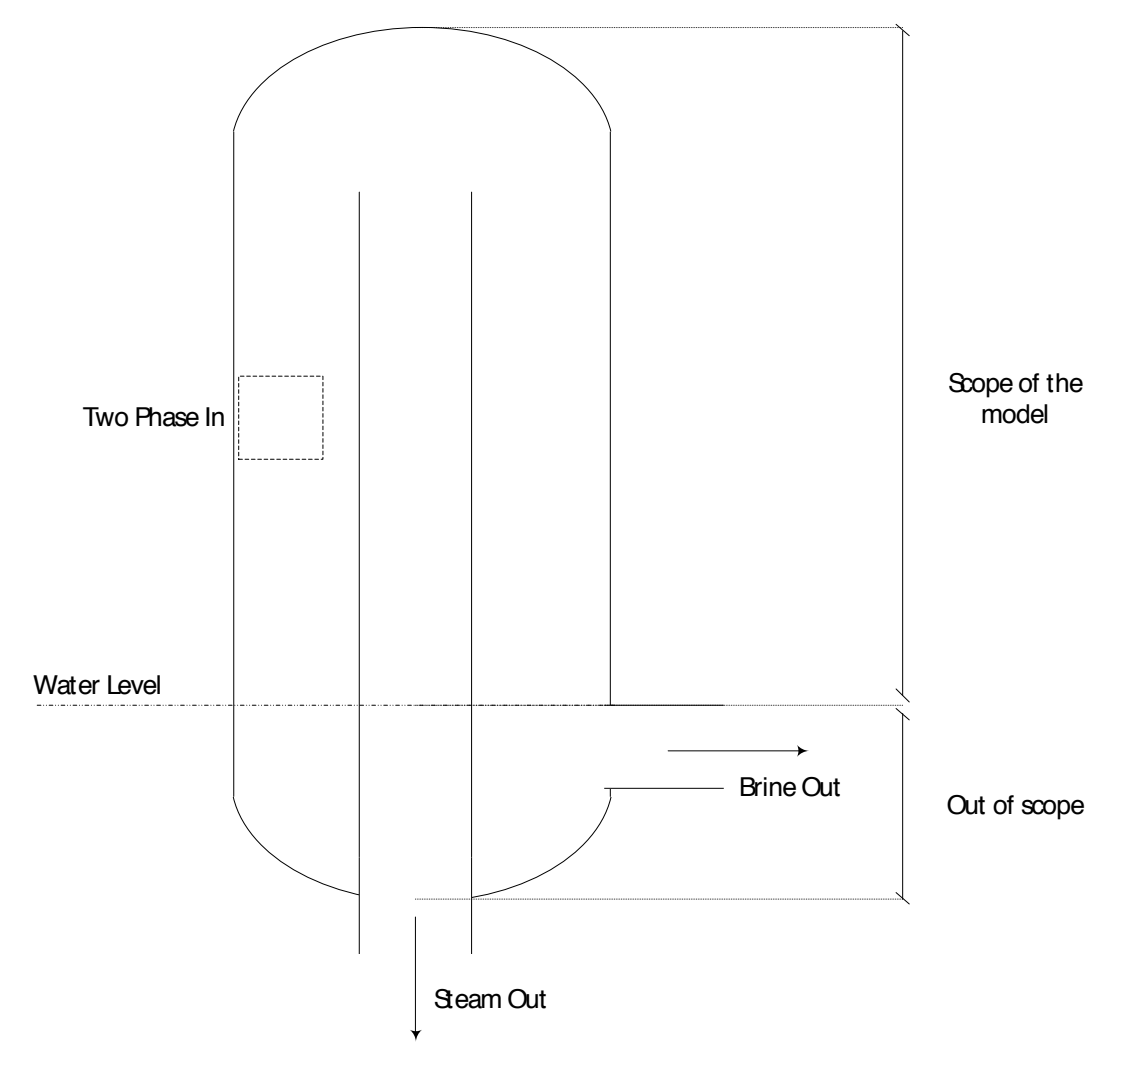
\includegraphics[width=0.68\linewidth]{../../figures/literature/purnanto-2013-model-scope.png}
\caption{Computational scope of the Purnanto et al.~ (2013) separator model. The domain ends at the assumed water level, leaving the lower vessel and brine outlet outside the model. Reproduced from Purnanto et al.~ (2013, p. 5, Figure 7).}\label{fig:purnanto-scope}
\end{figure}

Without a brine-removal path, steady mass balance would require all incoming liquid to leave through the steam outlet, which is inconsistent with the intended separation process. Addressing liquid removal and numerical convergence therefore became necessary before the effects of inlet conditions could be interpreted reliably. This formed an unexpected substantial part of the project involving tests of numerical liquid collectors and resolved brine-outlet treatments to assess whether they could support a mass-conserving solution that remained stable with further iteration.

The study covers the separator vessel and its inlet conditions, with emphasis on model reconstruction, liquid removal and numerical assessment. Downstream steam pipelines, condensate drain pots, scrubbers and demisters are outside its scope. Related simplified-domain investigations are discussed with attribution and with regard to differences in geometry and modelling choices.

The literature review establishes the physical and modelling context. The methods and verification sections explain how the calculations were performed and assessed. The results and discussion then examine their implications for the project objectives, followed by conclusions and recommendations for future work.
